\documentclass[a4paper,11pt,oneside]{report}
\usepackage[pdftex]{graphicx}
\usepackage[utf8x]{inputenc}
\usepackage[spanish]{babel}
\usepackage{fancyhdr}
\usepackage[Bjornstrup]{fncychap}
\usepackage{tabularx}
\usepackage{hyperref}
\usepackage{eurosym}
\usepackage{longtable}
\usepackage[table]{xcolor}
% \usepackage[usenames,dvipsnames]{color}
% \usepackage{colortbl}
% \usepackage[caption=false]{subfig}
% \usepackage{float}
% \usepackage{pdflscape}

\setlength{\headheight}{25pt}
\setlength{\parskip}{6pt}

% Margenes 1cm mas pequennos
% \addtolength{\oddsidemargin}{-1cm}
% \addtolength{\evensidemargin}{-1cm}
% \addtolength{\textwidth}{2cm}
% \addtolength{\voffset}{-1cm}
% \addtolength{\textheight}{2cm}

\lhead{
\includegraphics[height=20pt]{logo-umbrella.png}}
\chead{}
\rhead{\nouppercase{\leftmark}}

\hypersetup{
colorlinks,
citecolor=black,
filecolor=black,
linkcolor=black,
urlcolor=black
}

 % La que hay que liar para que las cabeceras de los capitulos
 % no tiren media pagina a la basura...

\makeatletter
\def\@makechapterhead#1{{
\parindent \z@ \raggedright \normalfont
\ifnum \c@secnumdepth >\m@ne
	\if@mainmatter
		\DOCH
	\fi
\fi
\interlinepenalty\@M
\if@mainmatter
	\DOTI{#1}
\else
	\DOTIS{#1}
\fi
}}

\def\@makeschapterhead#1{{
\parindent \z@ \raggedright
\normalfont
\interlinepenalty\@M
\DOTIS{#1}
}}
\makeatother

\begin{document}

\renewcommand\listtablename{Índice de tablas}
\renewcommand\tablename{Tabla}

\pagestyle{plain}

%%%% Title Page %%%%%

\pagenumbering{alph}

\begin{titlepage}
\begin{center}

% Logo

\includegraphics[width=0.6\textwidth]{logo-umbrella.png}\\[4cm]

% Title
{\huge \textbf{La Conquista del Mundo}}\\[0.5cm]
{\huge {Memoria del proyecto}}\\[4cm]

% Authors
\begin{minipage}{0.5\textwidth}
\large
\hspace{1cm}\textbf{\emph{Equipo de desarrollo}}\\
Ángel Durán Izquierdo\\
Antonio Gómez Poblete\\
Antonio Martín Menor de Santos\\
Daniel León Romero\\
Jorge Colao Adán\\
Laura Núñez Villa\\
Ricardo Ruedas García\\
\end{minipage}\\[2cm]

{\Large \today}
\end{center}
\end{titlepage}

%%%% end Title Page %%%%%

\clearpage
\pagenumbering{arabic}
\setcounter{page}{2}

\tableofcontents
\addcontentsline{toc}{chapter}{\contentsname}
% \listoffigures
% \listoftables

\clearpage

\pagestyle{fancy}

\chapter{Introducción}

\section{Descripción del juego}

\textit{La Conquista del Mundo} es un juego de estrategia por turnos que es
jugado sobre un tablero que representa el mapa del mundo. Este mapa está
dividido en 42 territorios.

Cada jugador comienza con un territorio y, por turnos, podrá realizar distintas
acciones como comprar nuevas unidades o territorios, o invadir territorios
enemigos. Todas estas acciones van dirigidas a alcanzar el objetivo del juego:
conquistar el mundo.

\section{Sistema distribuido}

La aplicación constituye un sistema distribuido. Los alumnos de la asignatura
formarán un total de cinco grupos. De éstos, uno de ellos se encargará del
desarrollo del servidor. El resto de grupos, entre los que se incluye éste,
realizarán independientemente clientes para este sistema.

Las comunicaciones entre las distintas aplicaciones se realizarán haciendo uso
del \textit{middleware} de comunicaciones RMI de Java. Para ello, se ha escrito
una interfaz común de clases para transmitir los datos entre los clientes y
el servidor.

\section{Visión general del documento}

% TODO

\chapter{Arquitectura}

La aplicación sigue una variación de la arquitectura de tres capas. Las capas
de presentación y dominio permanecen inalteradas. Sin embargo, esta aplicación
no necesita de almacenamiento externo, sino que se obtiene esta información
directamente del servidor. Por ese motivo, la capa de persistencia ha sido
sustituida por una capa de comunicaciones.

\begin{figure}[h]
\caption{Visión general de la arquitectura}
\centering
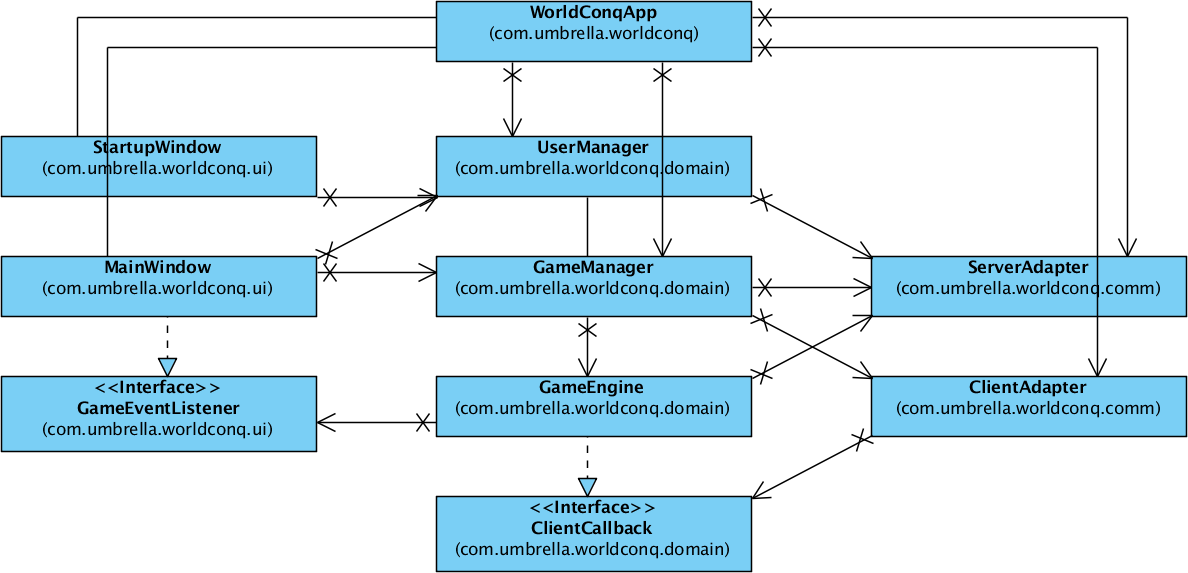
\includegraphics[scale=0.4]{img/ch02arch-overview.png}
\end{figure}

La visibilidad entre clases va de manera jerárquica, de manera que las clases
de presentación conocen a las de dominio, y las de dominio a las de
comunicaciones, pero no al revés. Para los casos en los que es necesario un
flujo de información en sentido contrario, se han creado interfaces para
desacoplar en la medida de los posible las capas inferiores.

La clase \texttt{WorldConqApp} es la única clase que no pertenece a ninguna de
las capas. Su función es la de ser el punto de entrada de la aplicación,
encargada de crear la estructura de clases, sus relaciones, y configurarlas a
partir de los parámetros de entrada.

\section{Capa de comunicaciones}

Esta capa contiene las clases \texttt{ServerAdapter} y \texttt{ClientAdapter}.
Ambas clases sirven de pasarela para los datos que fluyen entre el servidor y la
capa de dominio.

Estas clases incluyen una pequeña lógica de control. En el caso de la clase
\texttt{ServerAdapter}, ésta debe ser configurada con los datos del servidor
para así poder crear el \textit{proxy} a la interfaz remota. La ausencia de
esta configuración generará una excepción.

La clase \texttt{ClientAdapter} en cambio escucha todas las peticiones que
realiza el servidor sobre el cliente. Esta clase filtra estas peticiones de
acuerdo al juego activo en ese momento, descartando aquellas que no concuerden.

\section{Capa de dominio}

Esta capa está dividida en tres clases que se corresponden con los tres módulos
funcionales de la aplicación: gestión de usuarios, gestión de partidas, y motor
de juego.

La clase \texttt{UserManager} es la encargada de crear nuevas cuentas en la
aplicación y de mantener la información de la sesión activa. A esta clase
acceden el resto de clases para obtener la información sobre el jugador. De
manera análoga, la clase \texttt{GameManager} gestiona el listado, creación y
carga de partidas.

\begin{figure}[h]
\caption{Modelos de datos}
\centering
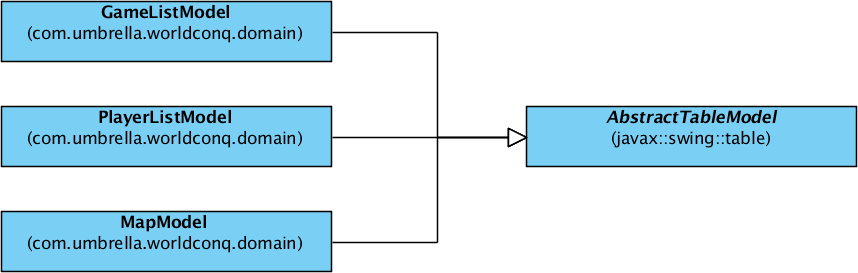
\includegraphics[scale=0.4]{img/ch02arch-models.png}
\end{figure}

Los datos de las partidas disponibles en el servidor son almacenados en objetos
de tipo \texttt{GameListModel}. Esta clase, y otras que se describen a
continuación, heredan de la clase \texttt{AbstractTableModel}. Esta clase
abstracta forma parte del \textit{framework} que proporciona Swing para
implementar el patrón arquitectónico Model-Vista-Controlador.

Hacer uso de este \textit{framework} significa que los accesos que hacen las
vistas a los modelos están definidos de antemano por una serie de interfaces.
Esto permite asociar clases disponibles en Swing con clases implementadas por el
equipo de trabajo de forma transparente.

En último lugar está el motor de juego, la clase \texttt{GameEngine}. Esta
clase se crea al comenzar a jugar a una partida e implementa toda la lógica de
dominio de una partida. Los datos con los que trabaja están almacenados en las
clases \texttt{PlayerListModel} y \texttt{MapModel}, los cuales heredan de la
clase \texttt{AbstractTableModel}, nombrada anteriormente.

\section{Capa de presentación}

En esta capa se encuentra la clase \texttt{StartupWindow}. Esta clase
representa a la primera ventana que se muestra. En ella, el usuario puede
registrar un nuevo usuario en el sistema y acceder con él.

Una vez accedido, se muestra la ventana principal, representada por la clase
\texttt{MainWindow}. Dentro de esta ventana existen dos modos de ejecución: el
modo de sala de espera y el modo partida.

\begin{figure}[h]
\caption{Vistas de datos}
\centering
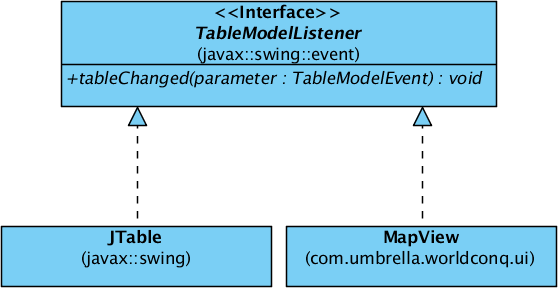
\includegraphics[scale=0.4]{img/ch02arch-views.png}
\end{figure}

En el modo de sala de espera, el usuario puede ver las partidas disponibles o
crear otras nuevas. Una vez se decida a cual jugar, la aplicación pasa a modo
partida.

La interfaz del modo partida se compone principalmente del mapa de juego. Junto
a él existen otro paneles informativos con los jugadores en la partida o una
lista con los últimos eventos.

Tanto las listas de partida como el mapa de juego implementan la interfaz
\texttt{TableModelListener}. Esto permite que estas clases puedan ser añadidas
como observadores de los cambios que sucedan en los modelos de datos.

\chapter{Desarrollo}

En este capítulo se hará un seguimiento del desarrollo completo del proyecto,
organizado por casos de uso. Para cada caso de uso, se comenzará hablando sobre
las decisiones de diseño tomadas. Un siguiente apartado tratará sobre cualquier
aspecto relevante de la implementación. Por último se mostrará un informe de
pruebas.

La documentación de este capítulo no sustituye al proyecto realizado con Visual
Paradigm, sino que destaca los aspecto más importantes para su mejor
comprensión.

\section{Caso de Uso: Registrarse}

\subsection*{Análisis y diseño}

\subsection*{Implementación}

\subsection*{Informe de pruebas}


\begin{itemize}
\item Nombre del \textit{tester} : Antonio Gómez Poblete
\item Fecha de asignación :  27 de Enero de 2011 
\item Fecha de finalización : 30 de Enero de 2011
\item Partes del código bajo prueba : UserManager::registerUser
\end{itemize}

A continuación se detallarán las pruebas de desarrollo (Pruebas unitarias con \textit{Junit}).

\begin{itemize}
\item Lista de los valores de prueba para cada atributo.
El criterio elegido para todos los valores de prueba (test data) ha sido: Añadir valores interesantes propensos a error (Conjetura de error). 
	\begin{enumerate}
	\item {\bf login:}  Cadena vacía, null, usuario existente y usuario no existente. 
	\item {\bf passwd:} Cadena vacía, null, cadena no vacía. 
	\item {\bf email:} Cadena vacía, null, cadena no vacía pero erronea: ([A-Za-z0-9][A-Za-z0-9\_\%-·]*, [A-Za-z0-9][A-Za-z0-9\_\%-·]*@, [A-Za-z0-9][A-Za-z0-9\_\%-·]*@[A-Za-z0-9][A-Za-z0-9\_\%-.]*, [A-Za-z0-9][A-Za-z0-9\_\%-·]*@[A-Za-z0-9][A-Za-z0-9\_\%-.]*.), cadena correcta ([A-Za-z0-9][A-Za-z0-9\_\%-·]*@[A-Za-z0-9][A-Za-z0-9\_\%-.]*.[A-Za-z0-9\_\%-]\{2,4\}). 	
\end{enumerate}
\item La estrategia para obtener los casos de prueba elegida ha sido \textit{each choice} y añadir algunos casos interesantes.

Para elegir tanto los valores de prueba como los casos de pruebas se ha analizado el comportamiento de este caso de uso (caja blanca). Tras este análisis se ha llegado a la conclusión de que hay en dos lugares en los que se pueden encontrar errores: Si al método registerUser se le da un parámetro erróneo (throw InvalidArgumentException), o si el nombre del usuario ya existe en el servidor (throw UserAlreadyExistsException). La primera comprobación es local, por ello si se lanza la excepcion InvalidArgumentException no se hará nada en el servidor y no se analizará si el usuario ya existe o no.

Además, si observamos las comprobaciones que se hacen en el cliente se ve que si login == null, independientemente del valor de los demás atributos se lanzará  InvalidArgumentException, por esa razón es independiente el valor de los demas atributos, lo que hace que muchos casos de prueba no sean necesarios de probar. Por otro lado, para probar qué pasa si el email es \textit{null} el resto de los parámetros deberán ser correctos, lo que añade algunos casos interesantes. Además de con \textit{null} lo comentado en este parrafo sucede con el resto de los parámetros. 


\item Teniendo en cuenta las consideraciones anteriormente mencionadas, la tabla completa de los casos de prueba y los  resultados esperados son:
\end{itemize}



\clearpage

{\footnotesize
\begin{longtable}[c]{l|c|c|c|c|c|}
 \textbf{Caso de prueba} & \textbf{login} & \textbf{passwd} & \textbf{email}
& \textbf{Objetivo del test} & \textbf{Resultado esperado} \\
\hline \hline
\endhead

testRegisterUser1 & vacío  & vacío   &  vacío  & login = vacío  & InvalidArgumentException\\
testRegisterUser2 & null  & null   &  null  & login = null  & InvalidArgumentException\\
testRegisterUser3 & JorgeCA  & jorge & jorge.colao@gmail.com & Usuario ya existente & UserAlreadyExistsException\\
testRegisterUser4 & JorgeCA & vacío & jorge.colao@gmail.com & passwd = vacío  & InvalidArgumentException\\
testRegisterUser5 & JorgeCA & null & jorge.colao@gmail.com & passwd = null  & InvalidArgumentException\\
testRegisterUser6 & JorgeCA & jorge & vacío & email = vacío  & InvalidArgumentException\\
testRegisterUser7 & JorgeCA & jorge & null & email = null  & InvalidArgumentException\\
testRegisterUser8 & JorgeCA & jorge & jorge & email = [A-Za-z0-9]& InvalidArgumentException\\
& & & & [A-Za-z0-9\_\%-·]* &\\
testRegisterUser9 & JorgeCA & jorge & jorge@ & email = [A-Za-z0-9]& InvalidArgumentException\\
& & & & [A-Za-z0-9\_\%-·]*@  &\\
testRegisterUser10 & JorgeCA & jorge & jorge@gmail & email = [A-Za-z0-9] & InvalidArgumentException\\
& & & & [A-Za-z0-9\_\%-·]*@  &\\
& & & & [A-Za-z0-9] &\\
& & & & [A-Za-z0-9\_\%-.]* &\\
testRegisterUser11& JorgeCA & jorge & jorge@gmail. & email = [A-Za-z0-9] & InvalidArgumentException\\
& & & & [A-Za-z0-9\_\%-·]*@  &\\
& & & & [A-Za-z0-9] &\\
& & & & [A-Za-z0-9\_\%-.]*. &\\
testRegisterUser12& LuisAn & luis & luis@gmail.com & email = [A-Za-z0-9] & \\
& & & & [A-Za-z0-9\_\%-·]*@  &\\
& & & & [A-Za-z0-9] &\\
& & & & [A-Za-z0-9\_\%-.]*. &\\
& & & & [A-Za-z0-9\_\%-]\{2,4\} &\\
\hline
\end{longtable}
}

A continuación se muestra un guión de pruebas exploratorias para cada uno de los escenarios posibles:
\begin{enumerate} 
\item Todos los datos son válidos y el usuario no existe.
	\begin{itemize}
	\item Acciones previas: El servidor debe estar funcionando y no tener un usuario con el nombre LuisAn.
	\item Acciones de prueba : En la ventana de inicio pinchamos en registrarnos y rellenamos el diálogo que nos aparecerá con los siguientes valores: LuisAn, luis, luis@gmail.com.
	\item Resultados esperados : Tras pulsar en aceptar  desaparecerá el diálogo de registro y en la parte superior de la ventana de inicio nos aparecerá en verde \emph {Usuario : LuisAn registrado"}.
	\end{itemize}
\item Todos los datos son válidos, pero el usuario existe.
	\begin{itemize}
	\item Acciones previas: El servidor debe estar funcionando y no tener un usuario con el nombre JorgeCA.
	\item Acciones de prueba : En la ventana de inicio pinchamos en registrarnos y rellenamos el diálogo que nos aparecerá con los siguientes valores: JorgeCA, jorge, jorge.colao@gmail.com.
	\item Resultados esperados : Tras pulsar en aceptar desaparecerá el diálogo de registro y en la parte superior de la ventana de inicio nos aparecerá en rojo \emph {El servidor indica: Error en el registro}.
	\end{itemize}

\item Algún dato introducido en el diálogo no es válido, independientemente de que el usuario exista o no.
	\begin{itemize}
	\item Acciones previas: El servidor debe estar funcionando.
	\item Acciones de prueba : En la ventana de inicio pinchamos en registranos y rellenamos el diálogo que nos aparecerá con los siguientes valores: JorgeCA, jorge, jorge@gmail..
	\item Resultados esperados : Tras pulsar en aceptar desaparecerá el diálogo de registro y aparecerá un panel de error mostrando \emph{Algún argumento es erroneo}. Despues de pulsar aceptar en el panel, volverá a aparecer el diálogo. Esto sucederá hasta que los datos sean correctos o demos a cancelar.  
	\end{itemize}
\end{enumerate} 

\section{Caso de Uso: Login}

\subsection{Análisis y diseño}

\subsection{Implementación}

\subsection{Informe de pruebas}

{\small
\begin{tabular}{r|l}
Nombre del \textit{tester} & Angel Durán Izquierdo \\
Fecha de asignación & 27 de enero de 2011 \\
Fecha de finalización & 2 de febrero de 2011 \\
Código bajo prueba & \texttt{UserManager::createSession}
\end{tabular}
}

\subsubsection{Pruebas de desarrollo}

A continuación se detallarán las pruebas de desarrollo (Pruebas unitarias con \textit{JUnit}).

Lista de los valores de prueba para cada atributo.
El criterio elegido para todos los valores de prueba (test data) ha sido: Añadir valores interesantes propensos a error (Conjetura de error).

\begin{itemize}
\item \textbf{\texttt{login}}
\subitem \textit{null}
\subitem Cadena vacía
\subitem Usuario existente: \texttt{Angel}
\subitem Usuario no existente: \texttt{ADuran}
\subitem Nombre de usuario registrado pero introducido con mayusculas: \texttt{ADuran}
\subitem Usuario existente con carácteres especiales: \texttt {Angel\&Duran}
\subitem Usuario existente con numeros: \texttt{1111, -1}

\item \textbf{\texttt{passwd}}
\subitem \textit{null}
\subitem Cadena vacía
\subitem Cadenas no vacías: \texttt{angel}
\subitem Cadenas con carácteres especiales: \texttt{22\&22}
\subitem Cadenas con numeros: \texttt{2222}

\end{itemize}

La estrategia para obtener los casos de prueba elegida ha sido
\textit{each choice} eligiendo los casos mas interesantes.

Para elegir tanto los valores de prueba como los casos de pruebas se ha analizado el comportamiento de este caso de uso (caja blanca). Tras este análisis se ha llegado a la conclusión de que hay en dos lugares en los que se pueden encontrar errores: Si al método createSession se le da un parámetro erróneo (throw InvalidArgumentException), o si el nombre del usuario no se ha registrado en el servidor (throw UserAlreadyExistsException).

Por otro lado se comprueba si al crear una sesion cuando ya se existía una, la anterior se cierra correctamente.


Teniendo en cuenta las consideraciones anteriormente mencionadas, la tabla completa de los casos de prueba y los resultados esperados son:

{\footnotesize
\begin{longtable}[c]{lccc}
 & \textbf{Valores de Prueba} & \textbf{Objetivo del test} & \textbf{Resultado esperado} \\
\hline \hline
\endhead

Test1 & (vacío, vacío)  & login-pass & InvalidArgument\\
Test2 & (Aduran, vacío) & pass & InvalidArgument\\
Test3 & (vacío, angel) & login & UserAlreadyExistst\\
Test4 & (Aduran, angel) & login-pass   & Sesión creada correctamente\\
Test5 & (null, angel) & login   & InvalidArgument\\
Test6 & (Aduran, null) & pass   & InvalidArgument\\
Test7 & (null, null) & login-pass   & InvalidArgument\\
Test8 & (ADuran, angel) & login & WrongLoginException\\
Test9 & (Aduran, Angel) & pass & WrongLoginException\\
Test10 & (1111, 22\&22) & login-pass & Sesión creada correctamente\\
Test11& (-1, 2222) & login-pass  & Sesión creada correctamente\\
Test12& (Angel\&Duran, angel) & login  &  Sesión creada correctamente \\
Test13 & (Aduran y ricki, angel y ricki) & Comportamiento createSession & Sesión creada correctamente\\
Test14 & (Aduran, angel) & Comportamiento createSession & RemoteException\\
Test15 & (Aduran, angel) & Comportamiento createSession & Sesión cerrada correctamente\\
Test16 & (Aduran, angel) & Comportamiento createSession & Sesión creada correctamente\\

\hline
\end{longtable}
}

\subsubsection{Pruebas exploratorias}

A continuación se muestra un guión de pruebas exploratorias para cada uno de los escenarios posibles:
\begin{enumerate}
\item El usuario esta registrado en el servidor
	\begin{itemize}
	\item Acciones previas: El servidor debe estar funcionando y el usuario debe estar registrado en el mismo.
	\item Acciones de prueba : En la ventana de inicio introducimos en el campo de Login la cadena Aduran y en el campo de Contraseña la cadena angel.
	\item Resultados esperados : Tras pulsar en aceptar la ventana de login desaparecerá y se abrirá la ventana de juego.
	\end{itemize}
\item El usuario no esta registrado en el servidor.
	\begin{itemize}
	\item Acciones previas: El servidor debe estar funcionando y no tener un usuario con el nombre ADuran.
	\item Acciones de prueba : En la ventana de login introducimos el usuario ADuran y la Contraseña angel.
	\item Resultados esperados : Tras pulsar en Aceptar aparece un mensaje de error en la parte superior de la ventana, este mensaje es: \emph {Contraseña o login Erroneos}.
	\end{itemize}

\item Falta algun dato por introducir.
	\begin{itemize}
	\item Acciones previas: El servidor debe estar funcionando.
	\item Acciones de prueba : En la ventana de login introducimos el nombre de usuario Aduran en el campo Login y dejamos el campo Contraseña vacío.
	\item Resultados esperados : Tras pulsar en Aceptar aparece un mensaje de error en la parte superior de la ventana, este mensaje es: \emph {Contraseña o login Erroneos}.
	\end{itemize}
\end{enumerate}


\chapter{Pruebas de desarrollo}

\section{Clase UserManager}

\subsection{UserManager::registerUser}

{\small
\begin{tabular}{r|l}
Nombre del \textit{tester} & Antonio Gómez Poblete \\
Fecha de asignación & 27 de enero de 2011 \\
Fecha de finalización & 30 de enero de 2011 \\
Código bajo prueba & \texttt{UserManager::registerUser}
\end{tabular}
}

A continuación se detallarán las pruebas de desarrollo (Pruebas unitarias con \textit{Junit}).

Lista de los valores de prueba para cada atributo.
El criterio elegido para todos los valores de prueba (test data) ha sido: Añadir valores interesantes propensos a error (Conjetura de error).

\begin{itemize}
\item \textbf{\texttt{login}}
\subitem \textit{null}
\subitem Cadena vacía
\subitem Usuario existente: \texttt{"JorgeCA"}
\subitem Usuario no existente: \texttt{"LuisAn"}

\item \textbf{\texttt{passwd}}
\subitem \textit{null}
\subitem Cadena vacía
\subitem Cadenas no vacías: \texttt{"jorge"}, \texttt{"luis"}

\item \textbf{\texttt{email}}
\subitem \textit{null}
\subitem Cadena vacía
\subitem Valores incorrectos: \texttt{"jorge"}, \texttt{"jorge@"}, \texttt{"jorge@gmail"}, \texttt{"jorge@gmail."}
\subitem Valores correctos: \texttt{"jorge.colao@gmail.com"}, \texttt{"luis@gmail.com"}
\end{itemize}

La estrategia para obtener los casos de prueba elegida ha sido
\textit{each choice} (Test 1 a 3 y 8 a 12 ) y añadir algunos casos
interesantes (Test 4 a 7).
El test 13 se ha elaborado para ver el comportamiento de registerUser cuando el servidor se ha desconectado.

Para elegir tanto los valores de prueba como los casos de pruebas se ha analizado el comportamiento de este caso de uso (caja blanca). Tras este análisis se ha llegado a la conclusión de que hay en dos lugares en los que se pueden encontrar errores: Si al método registerUser se le da un parámetro erróneo (throw InvalidArgumentException), o si el nombre del usuario ya existe en el servidor (throw UserAlreadyExistsException). La primera comprobación es local, por ello si se lanza la excepcion InvalidArgumentException no se hará nada en el servidor y no se analizará si el usuario ya existe o no.

Además, si observamos las comprobaciones que se hacen en el cliente se ve que si login == null, independientemente del valor de los demás atributos se lanzará  InvalidArgumentException, por esa razón es independiente el valor de los demas atributos, lo que hace que muchos casos de prueba no sean necesarios de probar. Por otro lado, para probar qué pasa si el email es \textit{null} el resto de los parámetros deberán ser correctos, lo que añade algunos casos interesantes. Además de con \textit{null} lo comentado en este parrafo sucede con el resto de los parámetros.


Teniendo en cuenta las consideraciones anteriormente mencionadas, la tabla completa de los casos de prueba y los resultados esperados son:

{\footnotesize
\begin{longtable}[c]{lccc}
 & \textbf{Valores de Prueba} & \textbf{Objetivo del test} & \textbf{Resultado esperado} \\
\hline \hline
\endhead

Test1 & (vacío, vacío, vacío)  & login & InvalidArgument\\
Test2 & (null, null, null) & login & InvalidArgument\\
Test3 & (JorgeCA, jorge, jorge.colao@gmail.com) & Usuario ya existente & UserAlreadyExistst\\
Test4 & (JorgeCA, vacío, jorge.colao@gmail.com) & passwd   & InvalidArgument\\
Test5 & (JorgeCA, null, jorge.colao@gmail.com) & passwd   & InvalidArgument\\
Test6 & (JorgeCA, jorge, vacío) & email   & InvalidArgument\\
Test7 & (JorgeCA, jorge, null) & email   & InvalidArgument\\
Test8 & (JorgeCA, jorge, jorge) & email & InvalidArgument\\
Test9 & (JorgeCA, jorge, jorge@) & email & InvalidArgument\\
Test10 & (JorgeCA, jorge, jorge@gmail) & email & InvalidArgument\\
Test11& (JorgeCA, jorge, jorge@gmail.) & email  & InvalidArgument\\
Test12& (LuisAn, luis, luis@gmail.com) & email  &  El usuario \\
& &  & queda registrado\\
Test13& (Angel\&Duran, angel, a@d.com)  & Comportamiento registerUser & RemoteException \\
\hline
\end{longtable}
}

\subsection{UserManager::login}

{\small
\begin{tabular}{r|l}
Nombre del \textit{tester} & Angel Durán Izquierdo \\
Fecha de asignación & 27 de enero de 2011 \\
Fecha de finalización & 2 de febrero de 2011 \\
Código bajo prueba & \texttt{UserManager::createSession}
\end{tabular}
}

A continuación se detallarán las pruebas de desarrollo (Pruebas unitarias con \textit{JUnit}).

Lista de los valores de prueba para cada atributo.
El criterio elegido para todos los valores de prueba (test data) ha sido: Añadir valores interesantes propensos a error (Conjetura de error).

\begin{itemize}
\item \textbf{\texttt{login}}
\subitem \textit{null}
\subitem Cadena vacía
\subitem Usuario existente: \texttt{Angel}
\subitem Usuario no existente: \texttt{ADuran}
\subitem Nombre de usuario registrado pero introducido con mayusculas: \texttt{ADuran}
\subitem Usuario existente con carácteres especiales: \texttt {Angel\&Duran}
\subitem Usuario existente con numeros: \texttt{1111, -1}

\item \textbf{\texttt{passwd}}
\subitem \textit{null}
\subitem Cadena vacía
\subitem Cadenas no vacías: \texttt{angel}
\subitem Cadenas con carácteres especiales: \texttt{22\&22}
\subitem Cadenas con numeros: \texttt{2222}

\end{itemize}

La estrategia para obtener los casos de prueba elegida ha sido
\textit{each choice} eligiendo los casos mas interesantes.

Para elegir tanto los valores de prueba como los casos de pruebas se ha analizado el comportamiento de este caso de uso (caja blanca). Tras este análisis se ha llegado a la conclusión de que hay en dos lugares en los que se pueden encontrar errores: Si al método createSession se le da un parámetro erróneo (throw InvalidArgumentException), o si el nombre del usuario no se ha registrado en el servidor (throw UserAlreadyExistsException).

Por otro lado se comprueba si al crear una sesion cuando ya se existía una, la anterior se cierra correctamente.


Teniendo en cuenta las consideraciones anteriormente mencionadas, la tabla completa de los casos de prueba y los resultados esperados son:

{\footnotesize
\begin{longtable}[c]{lccc}
 & \textbf{Valores de Prueba} & \textbf{Objetivo del test} & \textbf{Resultado esperado} \\
\hline \hline
\endhead

Test1 & (vacío, vacío)  & login-pass & InvalidArgument\\
Test2 & (Aduran, vacío) & pass & InvalidArgument\\
Test3 & (vacío, angel) & login & UserAlreadyExistst\\
Test4 & (Aduran, angel) & login-pass   & Sesión creada correctamente\\
Test5 & (null, angel) & login   & InvalidArgument\\
Test6 & (Aduran, null) & pass   & InvalidArgument\\
Test7 & (null, null) & login-pass   & InvalidArgument\\
Test8 & (ADuran, angel) & login & WrongLoginException\\
Test9 & (Aduran, Angel) & pass & WrongLoginException\\
Test10 & (1111, 22\&22) & login-pass & Sesión creada correctamente\\
Test11& (-1, 2222) & login-pass  & Sesión creada correctamente\\
Test12& (Angel\&Duran, angel) & login  &  Sesión creada correctamente \\
Test13 & (Aduran y ricki, angel y ricki) & Comportamiento createSession & Sesión creada correctamente\\
Test14 & (Aduran, angel) & Comportamiento createSession & RemoteException\\
Test15 & (Aduran, angel) & Comportamiento createSession & Sesión cerrada correctamente\\
Test16 & (Aduran, angel) & Comportamiento createSession & Sesión creada correctamente\\

\hline
\end{longtable}
}

\section{Clase GameManager}

{\small
\begin{tabular}{r|l}
Nombre del \textit{tester} & Jorge Colao Adán \\
& Daniel León Romero\\
Fecha de asignación & 18 de febrero de 2011 \\
Fecha de finalización & 21 de febrero de 2011 \\
Código bajo prueba & \texttt{GameManager}
\end{tabular}
}

En este apartado se hablará sobre las pruebas realizadas con la herramienta \textit{JUnit} sobre esta clase.

La estrategia a seguir para las pruebas de estos apartados será \textit{Each Choice}. La elección de los valores de los parámetos, se realizarán con valores límite para los atributos númericos y valores propensos a error para el resto.

\subsection{GameManager::updateGameList}

En este primer método como no tiene ningún parámetro lo que tenemos que comprobar es que al hacer el test con \textit{JUnit} no salte ninguna excepción. Además, comprobamos que inicialmente el número de partidas a las que se está unido y las partidas disponibles para unirse es igual a cero, y que después de la ejecución de este caso de uso es distinto de cero.

Debido a que con la herramienta \textit{JUnit} no podemos alcanzar una covertura alta, lo que haremos será hacer pruebas exploratorias.

\subsection{GameManager::createGame}

Este método tiene seis parámetros de entrada, por lo que tenemos que utilizar alguna estrategia de generación de casos de prueba. Hemos utilizado \textit{Each Choice} con la herramienta de la página \url{http://161.67.140.42/CombTestWeb/}. Pero comprobando las combinaciones que hemos obtenido nos hemos dado cuenta de que eran poco exahustivas (Test 1 a 4). Debido a este motivo, hemos añadido otros casos de prueba interesantes (Test 5 a 14), como son; probar para que falle cada parámetro independientemente.

Para elegir tanto los valores de prueba como los casos de pruebas de los casos interesantes se ha analizado el comportamiento de este método (mediante caja blanca). Después de analizar el método nos hemos dado cuenta de que solamente puede haber un tipo de error, que es "throw InvalidArgumentException". Esta comprobación es local, por ello si se lanza la excepcion InvalidArgumentException no se creará la partida en el servidor.

\begin{itemize}
\item \textbf{\texttt{name}}
\subitem \textit{null}
\subitem Cadena vacía
\subitem Cadena válida: \texttt{"partida"}

\item \textbf{\texttt{description}}
\subitem \textit{null}
\subitem Cadena vacía
\subitem Cadena válida: \texttt{"partida guerra mundo"}

\item \textbf{\texttt{gameSession}}
\subitem \textit{null}
\subitem Fecha errónea: \texttt{"01/Marzo/2009 a las 14:00"}
\subitem Fecha correctas: \texttt{"Hora actual"} y \texttt{"01/Marzo/2012 a las 14:00"}

\item \textbf{\texttt{turnTime}}
\subitem Número incorrecto: \texttt{"\--1"}
\subitem Número correcto. \texttt{"0"} y \texttt{"112"}

\item \textbf{\texttt{defTime}}
\subitem Número incorrecto: \texttt{"\--1"}
\subitem Número correcto. \texttt{"0"} y \texttt{"20"}

\item \textbf{\texttt{negTime}}
\subitem Número incorrecto: \texttt{"\--1"}
\subitem Número correcto. \texttt{"0"} y \texttt{"33"}
\end{itemize}

La única comprobación especial que podemos hacer es mirar si salta alguna excepción, si no salta ninguna excepción el método estará correcto, lo que creará una partida en el servidor.

Esta es la tabla de casos de prueba y resultados esperados.

{\footnotesize
\begin{longtable}[c]{lccc}
 & \textbf{Valores de Prueba} & \textbf{Objetivo del test} & \textbf{Resultado esperado} \\
\hline \hline
\endhead

Test1 & (vacío, vacío, null,  & name, gameSession & InvalidArgument\\
 & 112, 20, 33) & & \\
Test2 & (vacío, vacío, Fecha\_Actual, & name, defTime & InvalidArgument\\
 & 0, --1, 0) & & \\
Test3 & (null, "partida guerra mundo", & name, gameSession, & InvalidArgument\\
 &   Fecha\_Anterior, --1, --1, --1) & turnTime, defTime, negTime & \\
Test4 & ("partida", null,  & description   & InvalidArgument\\
 &  Fecha\_Posterior, 0, 0, 0) & & \\

Test5 & (vacío, vacío,  & name & InvalidArgument\\
 &  Fecha\_Posterior, 0, 0, 0) & & \\
Test6 & (null, "partida guerra mundo",  & name & InvalidArgument\\
 &   Fecha\_Posterior, 0, 0, 0) & & \\
Test7 & ("partida", null,  & description  & InvalidArgument\\
 &  Fecha\_Actual, 0, 0, 33) & & \\
Test8 & ("partida", "partida guerra mundo",  & gameSession & InvalidArgument\\
 &   Fecha\_Anterior, 0, 0, 33) & & \\
Test9 & ("partida", "partida guerra mundo",  & gameSession & InvalidArgument\\
 &   null, 0, 0, 33) & & \\
Test10 & ("partida", "partida guerra mundo",  & turnTime & InvalidArgument\\
 &   Fecha\_Actual, --1, 20, 33) & & \\
Test11 & ("partida", "partida guerra mundo",  & defTime & InvalidArgument\\
 &  Fecha\_Actual, 112, --1, 33) & & \\
Test12 & ("partida", "partida guerra mundo",  & negTime & InvalidArgument\\
 &  Fecha\_Actual, 112, 20, --1) & & \\
Test13 & ("partida", "partida guerra mundo",   & crear partida & Funcinamiento Correcto \\
 &  Fecha\_Actual, 112, 20, 33) & & \\
Test14 & ("partida", vacío,   & crear partida & Funcinamiento Correcto \\
 &  Fecha\_Posterior, 112, 20, 33) & & \\

\hline
\end{longtable}
}

\subsection{GameManager::joinGame}

Para este caso de uso tan sólo tenemos un parámetro que es el número del juego al que queremos unirnos. Por este motivo tenemos que comprobar los valores límite de la lista de partidas a unirse. Para representar los valores límite, hemos usado de límite inferior los números ''--1'' y "0", ya que la comparación es que sea menor de "0". Y para el límite superior usaremos el tope de partidas disponibles en el servidor y el tope más uno. En nuestro servidor tenemos dos partidas a las que nos podemos unir, por lo tanto, el tope sería ``1'' y el tope más uno sería ``2''. 

\begin{itemize}
\item \textbf{\texttt{gameSelected}}
\subitem Límite inferior: \texttt{"\--1"} y \texttt{"0"}
\subitem Límite superior: \texttt{"tope = 1"} y \texttt{"tope + 1 = 2"}
\end{itemize}

También tenemos que comprobar que antes de unirnos a la partida tiene que haber al menos una partida a la que podamos unirnos. Y después de unirnos comprobar que el número de filas en la lista de partidas actuales es mayor que antes y la lista de partidas para unirme es menor.

Esta es la tabla de casos de prueba y resultados esperados.

{\footnotesize
\begin{longtable}[c]{lccc}
 & \textbf{Valores de Prueba} & \textbf{Objetivo del test} & \textbf{Resultado esperado} \\
\hline \hline
\endhead

Test1 & (-1) & límite inferior & InvalidArgument\\
Test2 & (0) & primera partida & Funcionamiento correcto\\
Test3 & (0) & segunda partida & Funcionamiento correcto\\
Test4 & (2) & límite superior & InvalidArgument\\

\hline
\end{longtable}
}

\subsection{GameManager::connectToGame}

En este método tenemos dos parámetros, uno es el número de la partida seleccionada para jugar y el otro un evento, que para poder realizar la pruebas lo vamos a considerar ``null''. De esta forma, nos centramos en el primer parámetro que es el interesante. Como sólo tenemos un parámetro al igual que antes tenemos que sacar los valores límite. En esta ocasión en el servidor tenemos una única partida actual, por lo que el tope es ``0'' y el tope más uno es ``1''.

\begin{itemize}
\item \textbf{\texttt{gameSelected}}
\subitem Límite inferior: \texttt{"\--1"} y \texttt{"0"}
\subitem Límite superior: \texttt{"tope = 0"} y \texttt{"tope + 1 = 1"}
\end{itemize}

Además, antes de conectar tenemos que comprobar que almenos tengamos una partida a la cual podamos conectarnos para jugar y que el objeto GameEngine esté a null y que después de ejecutar el conectar no sea null.

Esta es la tabla de casos de prueba y resultados esperados.

{\footnotesize
\begin{longtable}[c]{lccc}
 & \textbf{Valores de Prueba} & \textbf{Objetivo del test} & \textbf{Resultado esperado} \\
\hline \hline
\endhead

Test1 & (-1) & límite inferior & InvalidArgument\\
Test2 & (0) & seleccionar partida & Funcionamiento correcto\\
Test3 & (1) & límite superior & InvalidArgument\\

\hline
\end{longtable}
}


\chapter{Pruebas exploratorias}

\section{Registrarse}

A continuación se muestra un guión de pruebas exploratorias para cada uno de los escenarios posibles:
\begin{enumerate}
\item Todos los datos son válidos y el usuario no existe.
	\begin{itemize}
	\item Acciones previas: El servidor debe estar funcionando y no tener un usuario con el nombre LuisAn.
	\item Acciones de prueba : En la ventana de inicio pinchamos en registrarnos y rellenamos el diálogo que nos aparecerá con los siguientes valores: LuisAn, luis, luis@gmail.com.
	\item Resultados esperados : Tras pulsar en aceptar  desaparecerá el diálogo de registro y en la parte superior de la ventana de inicio nos aparecerá en verde \emph {Usuario : LuisAn registrado"}.
	\end{itemize}
\item Todos los datos son válidos, pero el usuario existe.
	\begin{itemize}
	\item Acciones previas: El servidor debe estar funcionando y no tener un usuario con el nombre JorgeCA.
	\item Acciones de prueba : En la ventana de inicio pinchamos en registrarnos y rellenamos el diálogo que nos aparecerá con los siguientes valores: JorgeCA, jorge, jorge.colao@gmail.com.
	\item Resultados esperados : Tras pulsar en aceptar desaparecerá el diálogo de registro y en la parte superior de la ventana de inicio nos aparecerá en rojo \emph {El servidor indica: Error en el registro}.
	\end{itemize}

\item Algún dato introducido en el diálogo no es válido, independientemente de que el usuario exista o no.
	\begin{itemize}
	\item Acciones previas: El servidor debe estar funcionando.
	\item Acciones de prueba : En la ventana de inicio pinchamos en registranos y rellenamos el diálogo que nos aparecerá con los siguientes valores: JorgeCA, jorge, jorge@gmail..
	\item Resultados esperados : Tras pulsar en aceptar desaparecerá el diálogo de registro y aparecerá un panel de error mostrando \emph{Algún argumento es erroneo}. Despues de pulsar aceptar en el panel, volverá a aparecer el diálogo. Esto sucederá hasta que los datos sean correctos o demos a cancelar.
	\end{itemize}
\end{enumerate}

 \subsubsection{Iniciar sesión}

A continuación se muestra un guión de pruebas exploratorias para cada uno de los escenarios posibles:
\begin{enumerate}
\item El usuario esta registrado en el servidor
	\begin{itemize}
	\item Acciones previas: El servidor debe estar funcionando y el usuario debe estar registrado en el mismo.
	\item Acciones de prueba : En la ventana de inicio introducimos en el campo de Login la cadena Aduran y en el campo de Contraseña la cadena angel.
	\item Resultados esperados : Tras pulsar en aceptar la ventana de login desaparecerá y se abrirá la ventana de juego.
	\end{itemize}
\item El usuario no esta registrado en el servidor.
	\begin{itemize}
	\item Acciones previas: El servidor debe estar funcionando y no tener un usuario con el nombre ADuran.
	\item Acciones de prueba : En la ventana de login introducimos el usuario ADuran y la Contraseña angel.
	\item Resultados esperados : Tras pulsar en Aceptar aparece un mensaje de error en la parte superior de la ventana, este mensaje es: \emph {Contraseña o login Erroneos}.
	\end{itemize}

\item Falta algun dato por introducir.
	\begin{itemize}
	\item Acciones previas: El servidor debe estar funcionando.
	\item Acciones de prueba : En la ventana de login introducimos el nombre de usuario Aduran en el campo Login y dejamos el campo Contraseña vacío.
	\item Resultados esperados : Tras pulsar en Aceptar aparece un mensaje de error en la parte superior de la ventana, este mensaje es: \emph {Contraseña o login Erroneos}.
	\end{itemize}
\end{enumerate}


\section{Actualizar la lista de partida}

Guión de pruebas exploratorias para el método actualizar lista de partidas:

\begin{enumerate}
\item Pulsamos el botón ''Actualizar lista'', estando en hora para jugar una partida.
	\begin{itemize}
	\item Acciones previas: El servidor debe estar funcionando y habernos logeado con éxito.
	\item Acciones de prueba: Pulsamos el botón de ''Actualizar lista''.
	\item Resultados esperados: Tras pulsar el botón, aparecerán las dos litas de partidas, tanto las actuales (si estamos en hora) como las disponible para unirse (si no se han pasado la horas de juego y tiene territorios libres).
	\end{itemize}
\item Pulsamos el botón ''Actualizar lista'', no estando en hora para jugar una partida
	\begin{itemize}
	\item Acciones previas: El servidor debe estar funcionando y habernos logeado con éxito.
	\item Acciones de prueba: Pulsamos el botón de ''Actualizar lista''.
	\item Resultados esperados: Tras pulsar el botón, aparecen las partidas libres pero no las partidas actuales, ya que ho hay ninguna en hora.
	\end{itemize}
\end{enumerate}

\section{Crear una partida}

Guión de pruebas exploratorias para el método crear una partida:

\section{Unirse a una partida}

Guión de pruebas exploratorias para el método unirse a una partida:

\begin{enumerate}
\item Pulsamos el botón ''Unirse a la partida'', habiendo seleccionado una partida.
	\begin{itemize}
	\item Acciones previas: El servidor debe estar funcionando, habernos logeado con éxito y haber una partida libre disponible.
	\item Acciones de prueba: Seleccionamos una partida a la que queremos unirnos y luego pulsamos el botón de ''Unirse a la partida''.
	\item Resultados esperados: Si la partida a la que nos vamos a unir está en hora, nos saldra un mensaje para si queremos jugar. En cambio si no está en hora actualizará las dos listas.
	\end{itemize}
\item Pulsamos el botón ''Unirse a la partida'', sin haber seleccionado una partida.
	\begin{itemize}
	\item Acciones previas: El servidor debe estar funcionando, habernos logeado con éxito y haber una partida libre disponible.
	\item Acciones de prueba: Pulsamos el botón de ''Unirse a la partida''.
	\item Resultados esperados: La interfaz muestra un diálogo en el que indica que falta seleccionar una partida.
	\end{itemize}
\end{enumerate}

En realidad el fallo comprobado en la parte de Pruebas de desarrollo, no se puede dar porque la interfaz no lo permite.

\section{Conectarse a una partida}

Guión de pruebas exploratorias para el método conectarse a una partida:

\begin{enumerate}
\item Pulsamos el botón ''Conectarse a partida'', habiendo seleccionado una partida.
	\begin{itemize}
	\item Acciones previas: El servidor debe estar funcionando, habernos logeado con éxito y haber una partida disponible.
	\item Acciones de prueba: Seleccionamos la partida a la que queremos conectarnos para jugar y luego pulsamos el botón de ''Conectarse a partida''.
	\item Resultados esperados: Se cambia la interfaz mostrando la ventana de juego.
	\end{itemize}
\item Pulsamos el botón ''Conectarse a partida'', sin haber seleccionado una partida.
	\begin{itemize}
	\item Acciones previas: El servidor debe estar funcionando, habernos logeado con éxito y haber una partida disponible.
	\item Acciones de prueba: Pulsamos el botón de ''Conectarse a partida''.
	\item Resultados esperados: La interfaz muestra un diálogo en el que indica que falta seleccionar una partida.
	\end{itemize}
\end{enumerate}

En realidad el fallo comprobado en la parte de Pruebas de desarrollo, no se puede dar porque la interfaz no lo permite.



\end{document}
